\documentclass{article}
\usepackage[utf8]{inputenc}
\usepackage{siunitx}
\usepackage{graphics}
\usepackage[american,siunitx]{circuitikz}
\usepackage{amsmath}
\usepackage{svg} 
\usepackage{booktabs}
\usepackage{float}
\usepackage{xparse, xfp}
\usepackage{graphicx} 
\usepackage{steinmetz}
\usepackage{multirow}
\usepackage{pdfpages}
\usepackage{adjustbox}
%\renewcommand{\thesubsection}{\thesection.\alph{subsection}}
\newcommand{\equal}{=}
\newcommand*\circled[1]{\tikz[baseline=(char.base)]{
    \node[shape=circle,draw,inner sep=1pt] (char) {#1};}}

\title{ECE 2101L\\Electrical Circuit Analysis II Laboratory\\\,\\Lab 11\\Transfer Function of AC Circuits\\\,\\Report\\}
\author{Choi Tim Antony Yung}
%\author{Choi Tim Antony Yung\\\,\\Willis Nguyen\\Phineas Cozmiuc}

\begin{document}

\clearpage\maketitle
\thispagestyle{empty}
\newpage
\setcounter{page}{1}


\section{Circuit gain and phase shift for different frequencies}
\begin{center}
    \begin{adjustbox}{max width=\textwidth}
            \begin{circuitikz}
                \draw 
                    (0, 0) node[op amp] (opamp) {}
                    (opamp.-) -- ++(-0.5,0) to[R,l_=$R_1\equal\SI{3.3}{\kilo\ohm}$] ++(-2.5,0) to[V,l_=$V_{in}(\omega)$] ++(0,-2) -- ++(2,0) node[circ]{} node[ground](groundnode){} -- (groundnode |- opamp.+) -- (opamp.+)
                    (opamp.-) ++(-0.5,0) -- ++(0,1) coordinate (tempcoor) 
                    (tempcoor -| opamp.out) to[R,l_=$R_2\equal\SI{18}{\kilo\ohm}$] (tempcoor) -- ++(0,1.25) coordinate(temptempcoor) to[C,l=$C_2\equal\SI{0.68}{\micro\farad}$]  (temptempcoor -| opamp.out) -- (tempcoor -| opamp.out)
                    (tempcoor -| opamp.out) -- (opamp.out) -- ++(1.5,0) coordinate (voplus) to[R=$R_3\equal\SI{1.3}{\kilo\ohm}$, v=$V_{out}(\omega)$] (voplus |- groundnode) -- (groundnode)
                    ;
            \end{circuitikz}
    \end{adjustbox}
\end{center}

\subsection*{Procedure}
The above circuit was simulated with LTSpice XVII.

\subsection*{Result}
\begin{table}[H]
    \resizebox{\columnwidth}{!}{%
        \begin{tabular}{rrrrrrrrr}
            \toprule
            $f$ & $|H(\omega)|$ & $arg(H(\omega))$ & $|V_{out}|$ & $arg(V_{out})$ & $|V_{out}|$ & $arg(V_{out})$ & $|V_{out}|$ & $arg(V_{out})$ \\
            & calculated & calculated & calculated & calculated & measured & measured & error & error \\
            \midrule
            \SI{20 }{\hertz} & 2.973123  & 123.0296$^{\circ}$ & \SI{4.459684 }{\volt} & 123.0296$^{\circ}$ & \SI{4.45954 }{\volt} & 123.031$^{\circ}$ & 0.00\% & 0.00\% \\
            \SI{80 }{\hertz} & 0.8750748 & 99.23188$^{\circ}$ & \SI{1.312612 }{\volt} & 99.23188$^{\circ}$ & \SI{1.31259 }{\volt} & 99.2319$^{\circ}$ & 0.00\% & 0.00\% \\
            \SI{160}{\hertz} & 0.4418225 & 94.64609$^{\circ}$ & \SI{0.6627338}{\volt} & 94.64609$^{\circ}$ & \SI{0.662722}{\volt} & 94.6454$^{\circ}$ & 0.00\% & 0.00\% \\
            \SI{320}{\hertz} & 0.2214568 & 92.32687$^{\circ}$ & \SI{0.3321852}{\volt} & 92.32687$^{\circ}$ & \SI{0.33218 }{\volt} & 92.3251$^{\circ}$ & 0.00\% & 0.00\% \\
            \SI{640}{\hertz} & 0.1107969 & 91.16392$^{\circ}$ & \SI{0.1661954}{\volt} & 91.16392$^{\circ}$ & \SI{0.166193}{\volt} & 91.1603$^{\circ}$ & 0.00\% & 0.00\% \\
            \bottomrule    
        \end{tabular} }
\end{table}


\subsection*{Analysis}
At $f=\SI{80}{\hertz},$
$$H(2\pi80)=0.8750748\phase{99.23188}$$
$$V_{in}=1.5cos(2\pi80t+0)$$
$$V_{out}=1.312612cos(2\pi80t+99.23188^{\circ})$$
It can be observed that the amplitude of $V_{out}$ is the amplitude of $V_{out}$ multiplied by the magnitude of $H(\omega)$ and the phase of $V_{out}$ is the phase of $V_{out}$ added by the phase of $H(\omega)$.

\newpage
\begin{figure}[H]
    \centering
        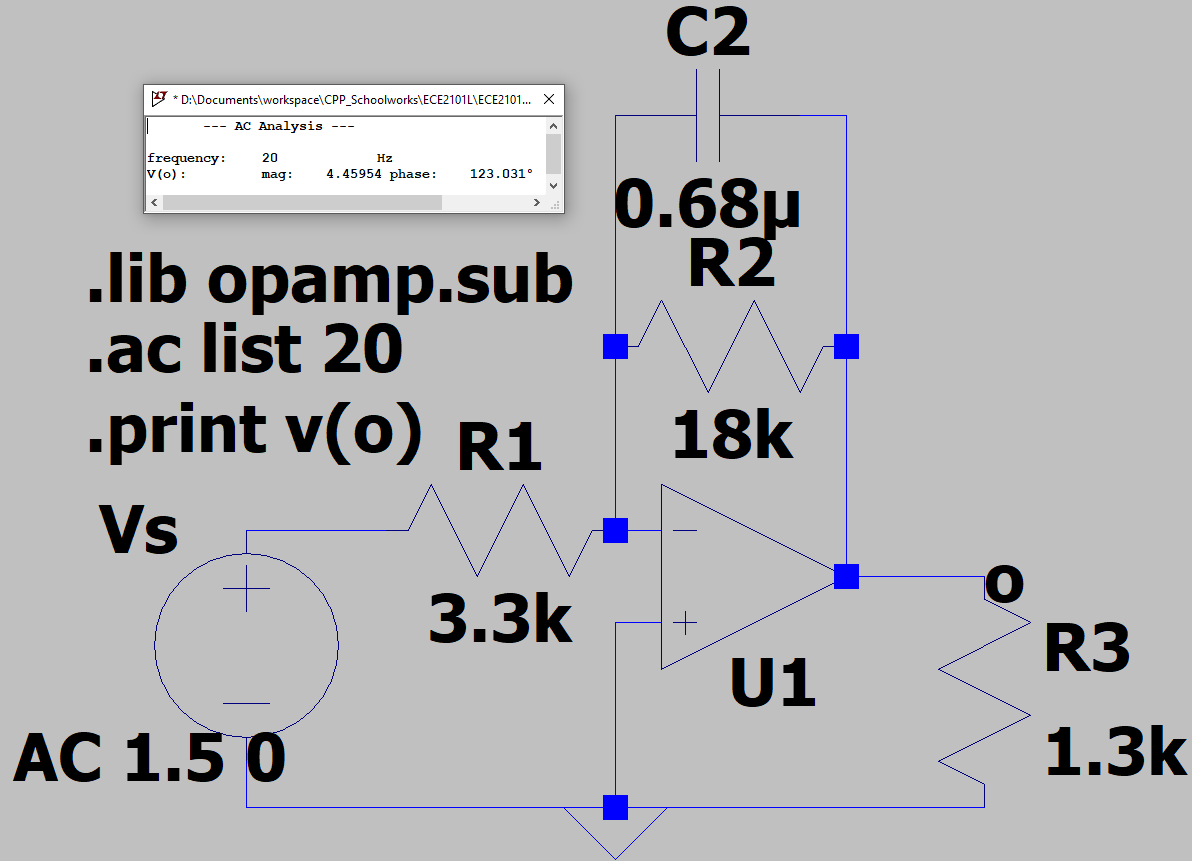
\includegraphics[width=\textwidth]{ECE2101L_Lab11_B1.png}
        \caption{Simulation of the circuit with LTSpice XVII at $f=\SI{20}{\hertz}$}
\end{figure}
\begin{figure}[H]
    \centering
        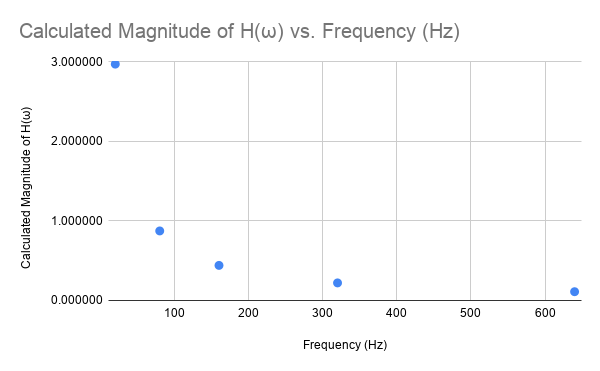
\includegraphics[scale=0.45]{ECE2101L_Lab11_B1_plot1.png}
        \caption{Calculated Magnitude of $H(\omega)$ vs. Frequency (Hz)}
\end{figure}
\begin{figure}[H]
    \centering
        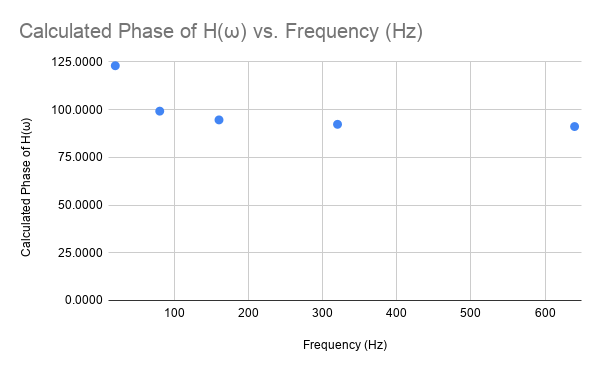
\includegraphics[scale=0.45]{ECE2101L_Lab11_B1_plot2.png}
        \caption{Calculated Phase of $H(\omega)$ ($^{\circ}$) vs. Frequency (Hz)}
\end{figure}
\begin{figure}[H]
    \centering
        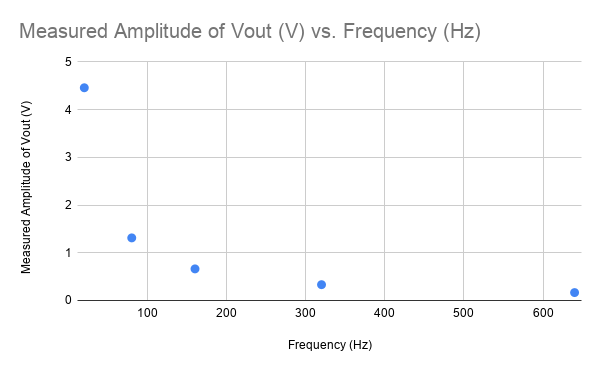
\includegraphics[scale=0.45]{ECE2101L_Lab11_B1_plot3.png}
        \caption{Measured Amplitude of $V_{out}$ (V) vs. Frequency (Hz)}
\end{figure}

\newpage

\section{Circuit maximum gain and phase shift}

\subsection*{Result}
\begin{table}[H]
    \resizebox{\columnwidth}{!}{%
    \begin{tabular}{cccccc}
        \toprule
        Frequency & \multicolumn{2}{c}{Gain} & \multicolumn{2}{c}{Phase shift} \\
        Hz& maximum & minimum & maximum & minimum \\
        \midrule
        0 & \SI{8.18129}{\volt} & & 180$^{\circ}$ & \\
        $+\infty$ & & \SI{0}{\volt} & & 90$^{\circ}$ \\ 
        \bottomrule
    \end{tabular} }
\end{table}

\subsection*{Analysis}
$$H(\omega)=\frac{1}{\sqrt{(\frac{R_1}{R_2})^2+(R_1(2\pi f)C_2)^2}}\phase{tan^{-1}\left(-R_2(2\pi f) C_2\right)}$$
From the equation above we can determine that the gain is maximized when the denominator is minimized, which is when the frequency goes to zero. Also, the gain minimizes when the denominator is maximized, which is when frequency approaches positive infinity. 

Assuming the range of $tan^{-1}(x)$ is $[90^{\circ},180^{\circ}]$ when $x$ is not positive, the maximum and minimum phase shift can also be determined from the above equation; $tan^{-1}(x)$ is at its maximum $=180^{\circ}$ when $x=-R_2(2\pi f) C_2$ goes to zero, which is when f goes to zero. Also, $tan^{-1}(x)$ is at its minimum $=90^{\circ}$ when $x=-R_2(2\pi f) C_2$ approaches positive infinity, which is when f approaches positive infinity.

\newpage

\end{document}

